%!TeX root=../tese.tex
%("dica" para o editor de texto: este arquivo é parte de um documento maior)
% para saber mais: https://tex.stackexchange.com/q/78101/183146

% Vamos definir alguns comandos auxiliares para facilitar.

% "textbackslash" é muito comprido.
% \newcommand{\sla}{\textbackslash}

% Vamos escrever comandos (como "make" ou "itemize") com formatação especial.
% \newcommand{\cmd}[1]{\textsf{#1}}

% Idem para packages; aqui estamos usando a mesma formatação de \cmd,
% mas poderíamos escolher outra.
% \newcommand{\pkg}[1]{\textsf{#1}}

% A maioria dos comandos LaTeX começa com "\"; vamos criar um
% comando que já coloca essa barra e formata com "\cmd".
% \newcommand{\ltxcmd}[1]{\cmd{\sla{}#1}}

\chapter{Static Analysis}
\label{cap:static}

Understanding how social networks recommend content to users is central to the
debate around political polarization and radicalization. There are many ways of
exploring recommender systems without examining their code \citep{}, from
simulating their behavior after careful observation to directly collecting
recommendation data, but most of them allow us to examine only one perspective
of the algorithm at a time. This means that studying a social network's
recommendation technique has inherent limitations.

Most of the algorithms currently employed by social media companies are trade
secrets. They are also subject to constant experimentation and tuning \citep{},
which might render worthless any research performed before an update to the
algorithm, no matter how careful the design of the study was.

With our experiments we aim to make a tangible contribution to the field of
recommender systems, specifically how their design might (or might not) foster
confinement dynamics and create degenerate ``feedback loops''. If the main
hypothesis is confirmed, this could mean that even a relatively small fraction
of the content can tip the algorithm in its favor, amplifying their message,
creating filter bubbles, and possibly sending users on a radicalization spiral
if that topic is related to politics or other contentious subjects.

In this chapter we will analyze a recommendation system statically, that is,
without taking into account its evolution after multiple rounds of training and
learning from new data. This step is essential insofar as it generates valuable
information to better orient our dynamic analyses.

\section{Datasets}
\label{sec:datasets03}

Before discussing any experiment, it is necessary to introduce the datasets used
in the models. The main dataset explored in this dissertation is MovieLens
\citep{harper_movielens_2015}, a well-known set of movie reviews that has been
featured in many recommender system tutorials and papers for the past few years.
The full dataset, with 27,000,000 ratings applied to 58,000 movies, was enriched
by \citet{banik_movies_2017} with information about the movies' credits,
metadata, keywords, and links. In the end, because of technical limitations, the
dataset used in this chapter was sampled until 30,689 movies were left; this was
the largest dataset that could be processed in less than one hour by the
hardware we had access to.

The second dataset, used for validation purposes only, was the Book-Crossing
Dataset \citep{ziegler_book-crossing_2004}. Just like the enriched MovieLens,
this dataset contained entries for ratings (1,149,780) applied by users
(278,858) to items (271,379 books), and information about these items like
title, author, publisher, etc.

\section{Experiments}
\label{sec:experiments}

The static analysis involved crafting many different models and analyzing their
recommendations as a whole. The goal of these experiments was to test the
hypothesis that even a simple recommendation algorithm could demonstrate some
sort of bias towards a subset of the items being recommended. More specifically,
given an algorithm that is user agnostic, i.e., that cannot be influenced by
users' personal preferences, would the resulting recommender system favor some
item? Excluding user information is important because, as demonstrated by
\citet{stoica_algorithmic_2018}, users might have their own biases and these
could get transferred on to the model; the objective here is understanding the
algorithm by itself without external influences.

% Some preliminary experiments were conducted in order to gather some evidence in
% favor or against the main hypothesis being tested. In total, fifteen different
% recommendation models were trained and analyzed, with each plot below
% representing one of these models. For simplicity's sake, even though all models
% represented here are non-parametric, we still say they were ``trained'' because
% the datasets used to generate recommendations are different.

To evaluate the recommendation models, at least qualitatively, we can compare
their ``recommendation profiles'': a summary of how many times every item is
recommended overall. To create this profile, the model is asked to return the
top-$n$ most similar items to the input according to its internal similarity
metric, and this process is repeated for every item in the dataset. The
recommendation profile of the model is the number of times each item showed up
in the top-$n$ most similar items of the whole dataset.

For example, a recommendation algorithm applied the present version of the
MovieLens dataset would generate a list of $n$ movies for each input, creating a
list of $30,689 \times n$ movies. This operation is very costly, approaching
$O(MN)$ complexity, where $M$ is the number of users in the dataset and $N$ is
the total number of available numbers. After this computationally intensive
calculation, the occurrence of each ID would be counted and ranked accordingly
to facilitate interpretation of results, that is, the movie ranked number 1
would be the movie featured the most times in the set of all recommendations,
and so forth for every other rank. From now on $n$ will be fixed to 10, which
is, on average, roughly how many videos YouTube shows on its recommendation
sidebar.

The first model examined is the ``trivial model'', which is a simple sampler
that returns $n$ movies at random when asked for a recommendation. Its
recommendation profile can be seen in Figure~\ref{fig:fig1} and, logically, the
number of times each movie is recommended approaches a normal distribution and,
therefore, the recommendation profile also approaches the cumulative
distribution function (CDF) of said distribution. The most recommended movie
appeared 25 times in the final list, while the least recommended movie did not
appear at all. Figure~\ref{fig:fig1b} shows the log-log plot of the
recommendation profile.

\begin{figure}
  \centering
  \begin{subfigure}{0.45\textwidth}
    \centering
    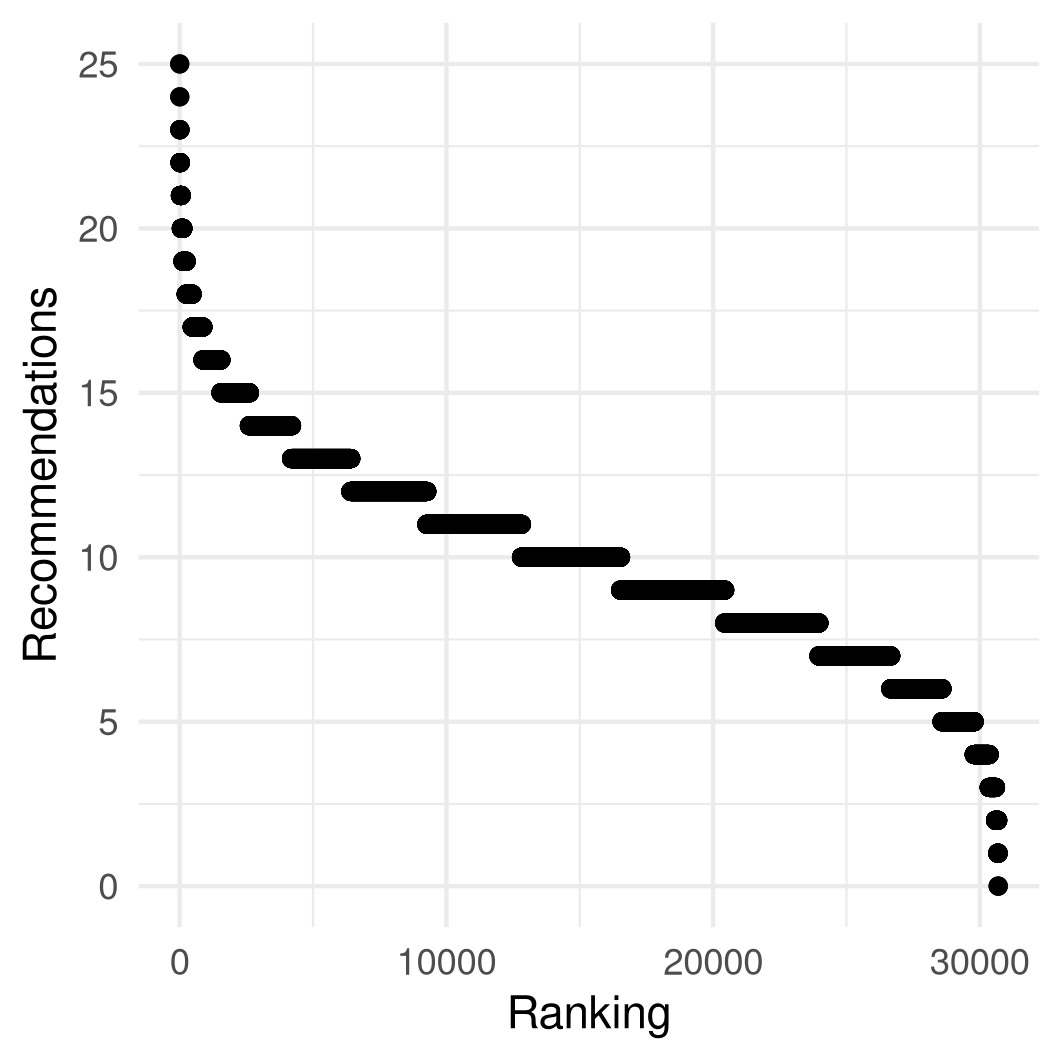
\includegraphics[width=\textwidth]{1a_random}
    \caption{Recommendation profile.\label{fig:fig1a}}
  \end{subfigure}
  \begin{subfigure}{0.45\textwidth}
    \centering
    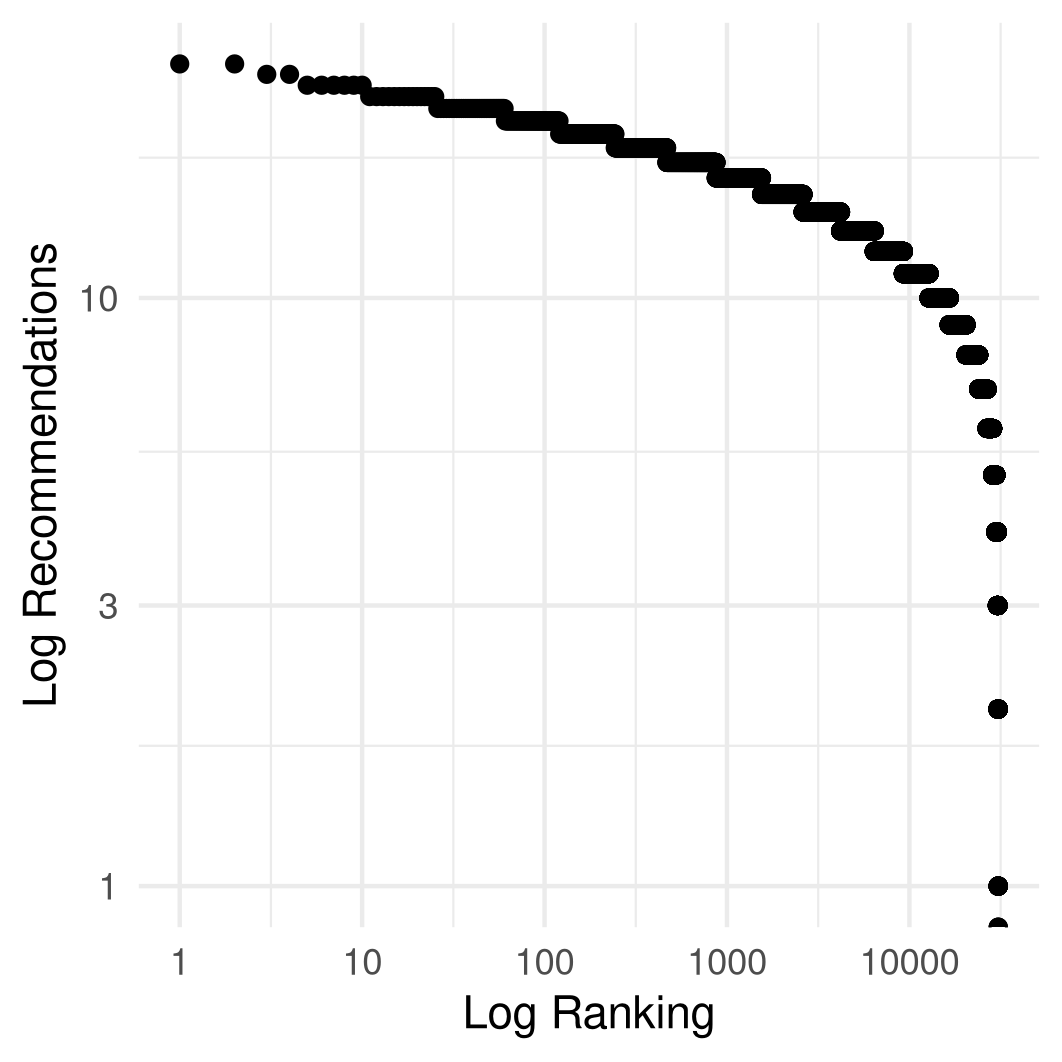
\includegraphics[width=\textwidth]{1b_random_log}
    \caption{Log-log plot.\label{fig:fig1b}}
  \end{subfigure}
  \caption{Recommendation profile for the trivial model (a) and log-log plot
    (b).\label{fig:fig1}}
\end{figure}

Besides the trivial model, the simplest model that excludes user information is
the content-based recommender. In the real world this is an algorithm that is
able to identify similar items based on their metadata (description, tags, etc.)
and suggest the closest items to the one being purchased or viewed. A
straightforward way of building such an algorithm is creating a vector
representation of each item and then using a similarity metric to recommend the
items most similar to the one in question. The chosen similarity metric was
cosine similarity because of its simplicity, robustness, and ubiquity
\citep{sarwar_item-based_2001}.

The main non-trivial model used in this study was the one that simply generated
vector representations for the full MovieLens dataset, without any modifications
(which is why it will henceforth be referred to as the ``vanilla model''). The
metadata for each movie was made up of its keywords, main cast, director, and
genres. The vector transformation was very simple, with each position
representing one of the words of the corpus, and each element indicating how
many times that word appeared in the metadata for that movie. When the
recommendation for a movie was requested, the algorithm measured the cosine
similarity between it and every other movie, returning the IDs belonging to
the top $n = 10$ most similar vectors.

The recommendation profile for the vanilla model can be seen in
Figure~\ref{fig:fig2a}. Here, the movie ranked number 1 appeared more than 2000
times in the full list of recommendations, with an almost exponential decrease
in the number of appearances from then on, as made evident by the log-log plot
on Figure~\ref{fig:fig2b}. This recommendation profile is a big departure from
the trivial model discussed above.

\begin{figure}
  \centering
  \begin{subfigure}{0.45\textwidth}
    \centering
    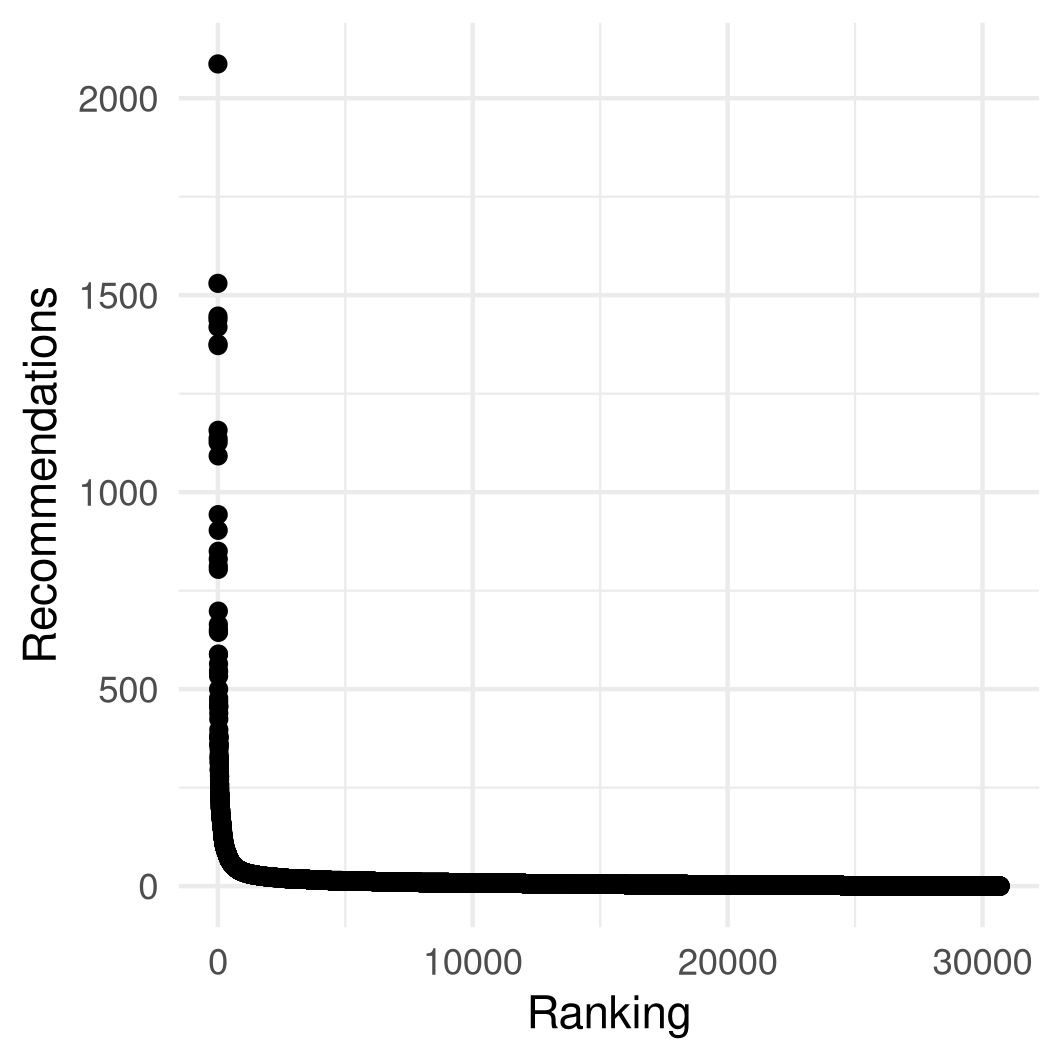
\includegraphics[width=\textwidth]{2a_vanilla}
    \caption{Recommendation profile.\label{fig:fig2a}}
  \end{subfigure}
  \begin{subfigure}{0.45\textwidth}
    \centering
    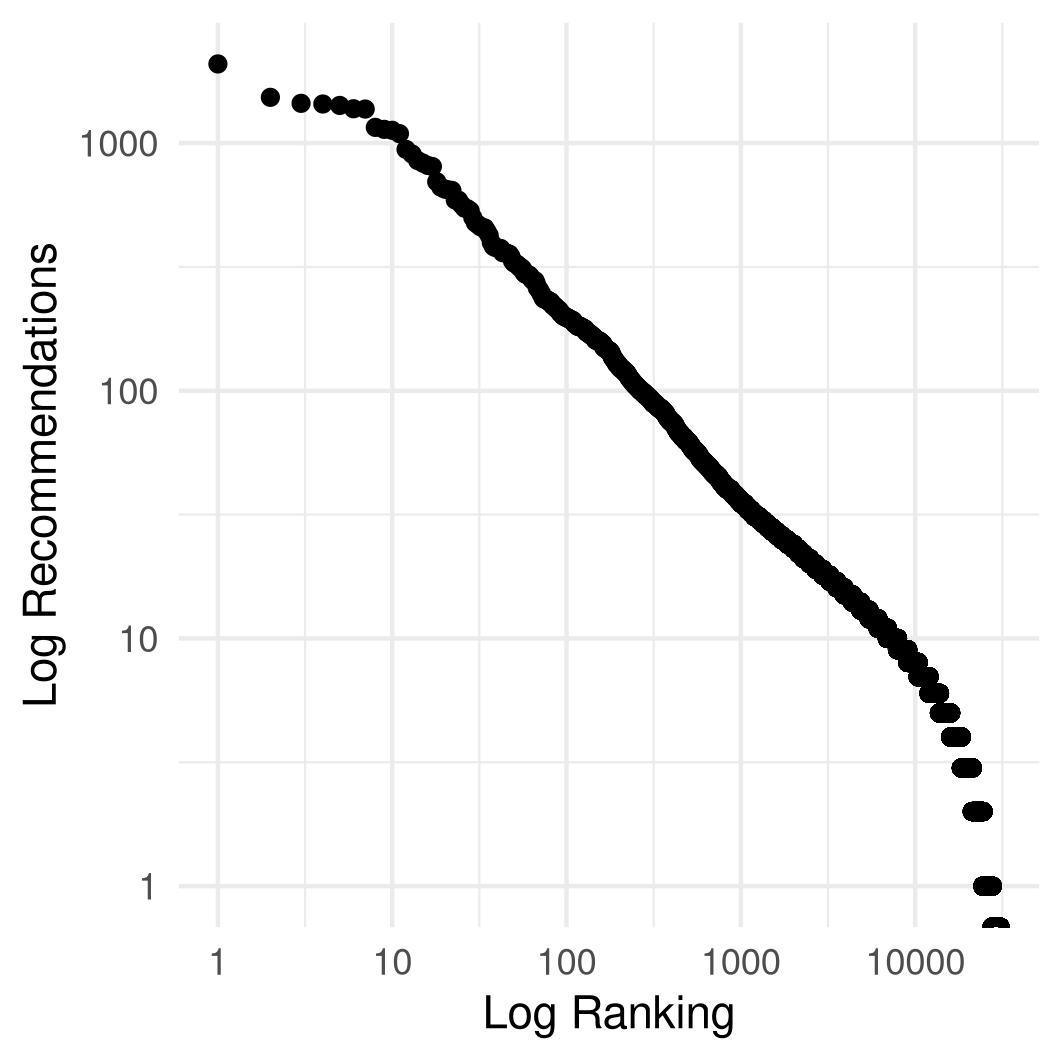
\includegraphics[width=\textwidth]{2b_vanilla_log}
    \caption{Log-log plot.\label{fig:fig2b}}
  \end{subfigure}
  \caption{Recommendation profile for the vanilla model (a) and log-log plot
    (b).\label{fig:fig2}}
\end{figure}

% Precisa, sem falta, colocar uma distribuição das notas dos filmes para mostrar
% que, apesar de existirem filmes mais populares, eles não são exponencialmente
% mais populares. Isso justifica procurar outra explicação para a diferença
% entre o vanila e o trivial que não seja somente o rating dos filmes.

A potential explanation for the difference between trivial and vanilla could
reside in the least used terms in the metadata: movies whose metadata share rare
words might have been recommended less frequently than movies whose metadata are
not so unique. To test this hypothesis, a cutoff point was created for words to
be included in the vector representation of the movies. Three cutoff points were
tested and only words with an absolute frequency larger than or equal to $k$, $k
= {2, 5, 8}$, could be included in the vector representations. The results can
be seen in Figure~\ref{fig:fig3} and, aside from variations in the
$y$-intercept, all plots are qualitatively very similar to
Figure~\ref{fig:fig2a}, indicating that rare words probably are not to blame for
the exponential-like decay.

\begin{figure}
  \centering
  \begin{subfigure}{0.3\textwidth}
    \centering
    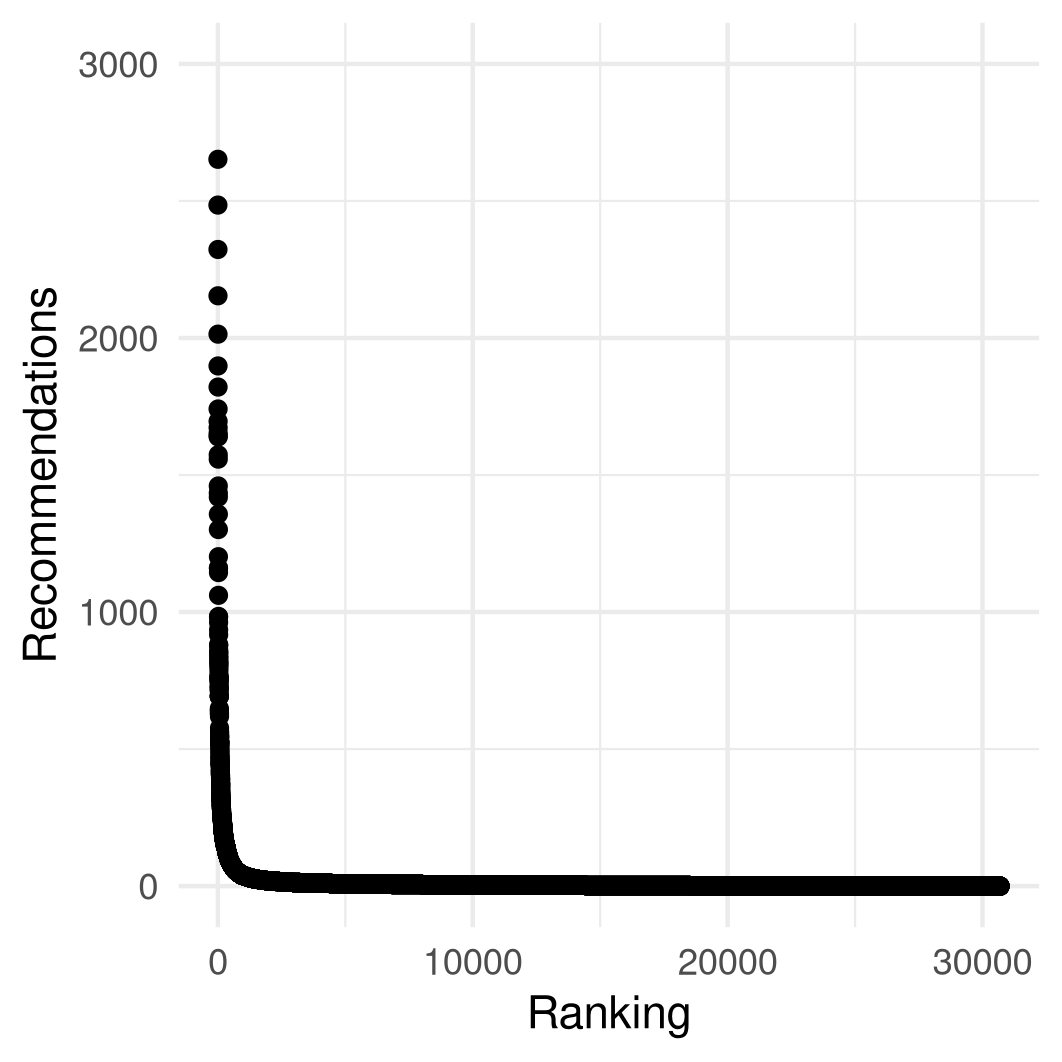
\includegraphics[width=\textwidth]{3a_cutoff_low}
    \caption{Cutoff $k = 2$.\label{fig:fig3a}}
  \end{subfigure}
  \begin{subfigure}{0.3\textwidth}
    \centering
    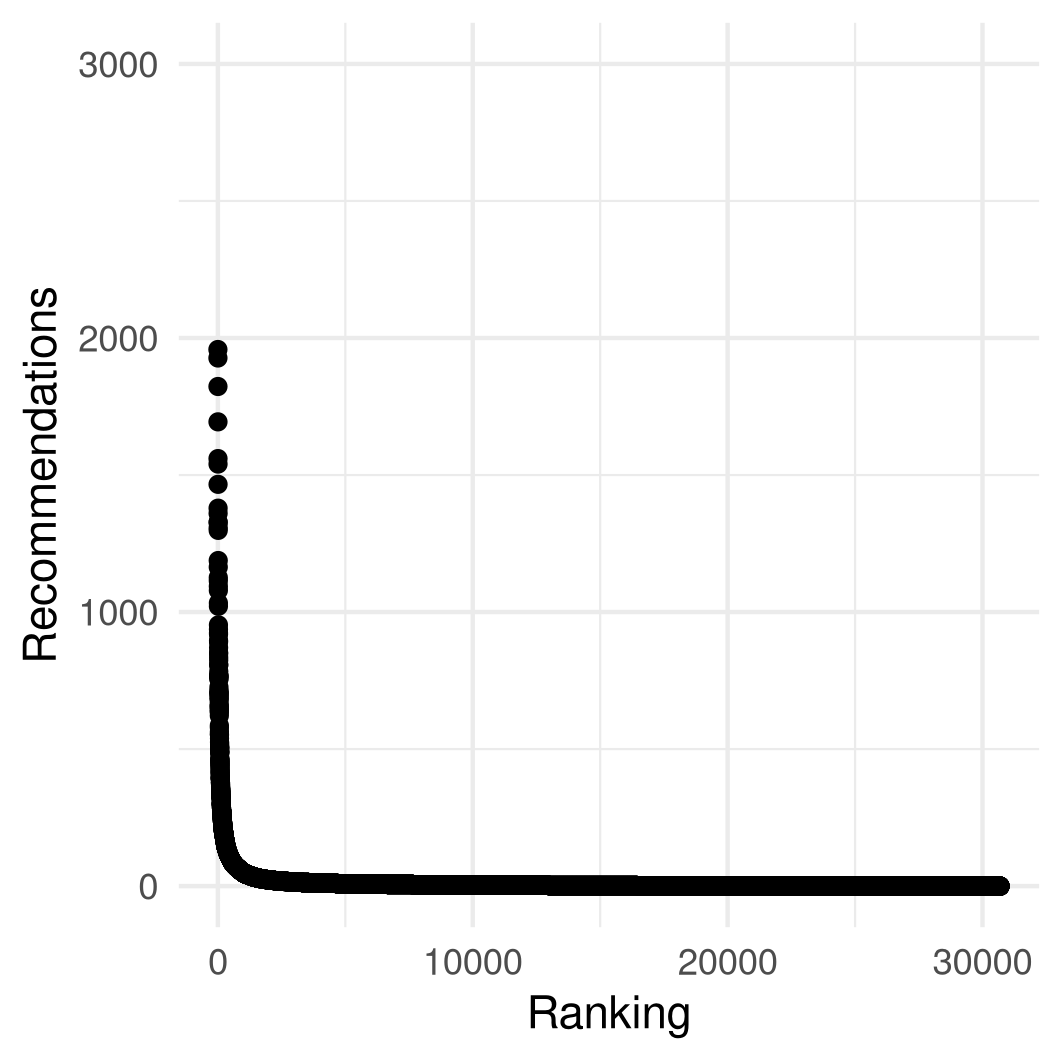
\includegraphics[width=\textwidth]{3b_cutoff_med}
    \caption{Cutoff $k = 5$.\label{fig:fig3b}}
  \end{subfigure}
  \begin{subfigure}{0.3\textwidth}
    \centering
    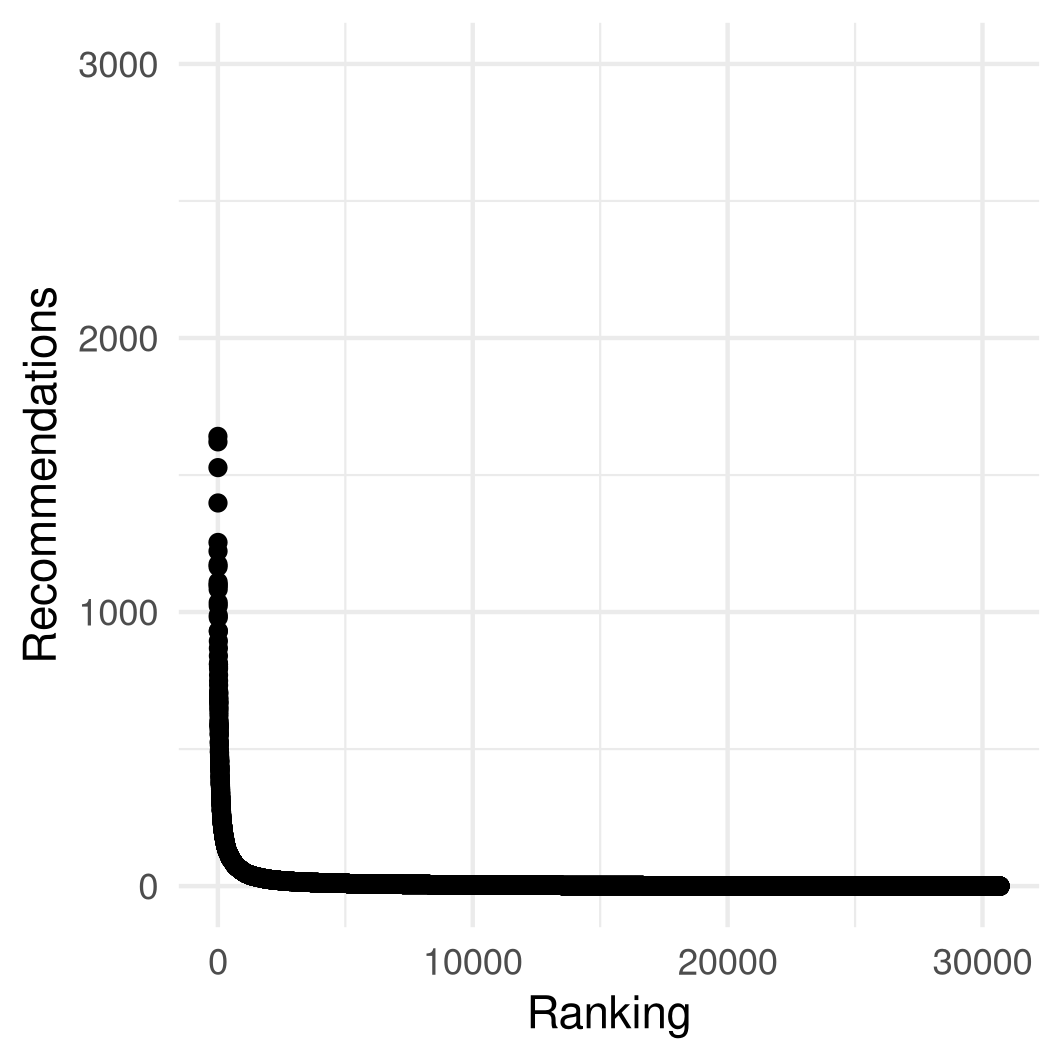
\includegraphics[width=\textwidth]{3c_cutoff_high}
    \caption{Cutoff $k = 8$.\label{fig:fig3c}}
  \end{subfigure}
  \caption{Recommendation profile for cutoff $k = 2$ (a), $5$ (b), and $8$
    (c).\label{fig:fig3}}
\end{figure}

The second validation experiment involved attempting to use other distance
metrics instead of cosine similarity \citep{ricci_introduction_2011}, since that
could also be a source of the strange behavior of the recommendation profile.
The goal here was to verify whether other metrics could do a better job at not
creating a subset of movies that ended up exponentially more recommended than
the rest.

Figure~\ref{fig:fig4} showcases a comparison between cosine distance, euclidean
distance and manhattan distance. It is clear that there are no meaningful
differences between the recommendation profiles generated by each metric.

\begin{figure}
  \centering
  \begin{subfigure}{0.3\textwidth}
    \centering
    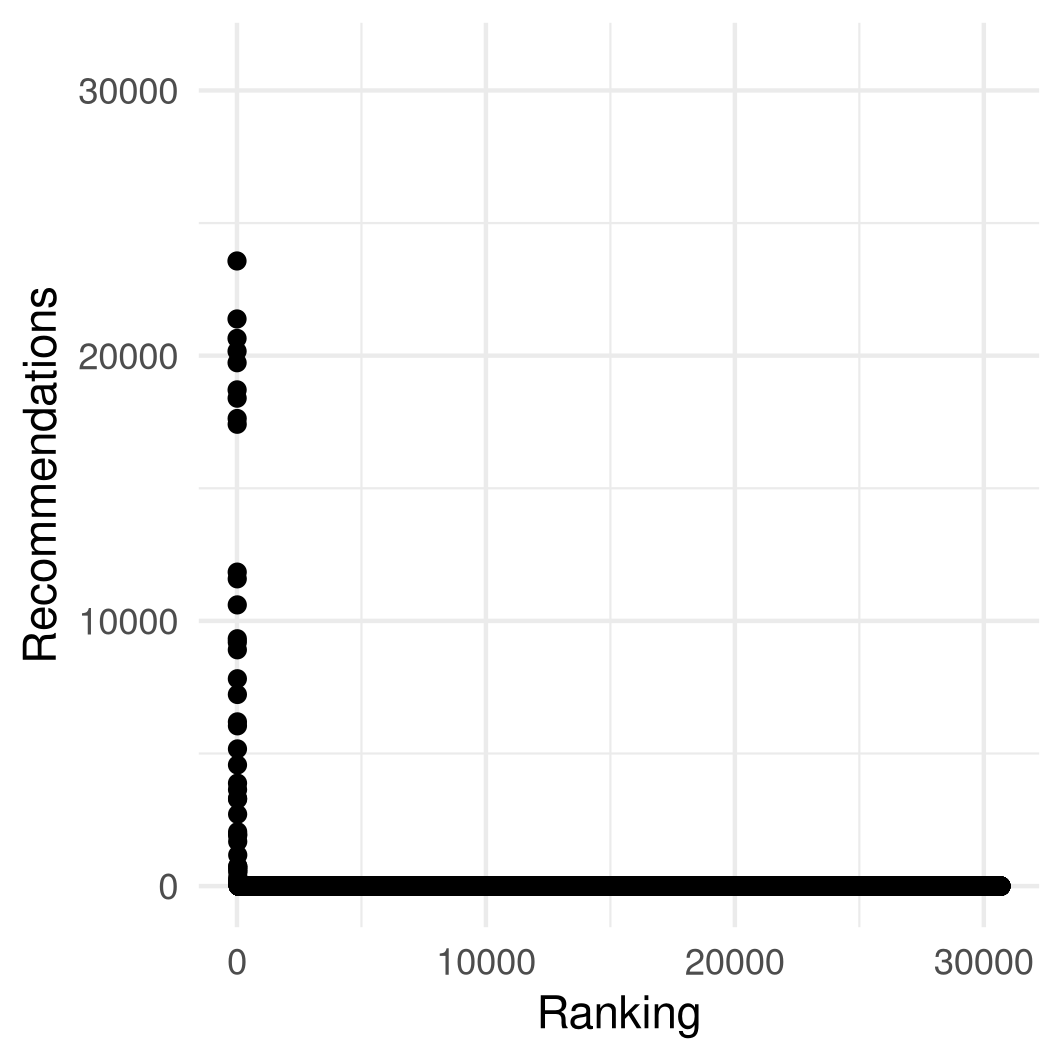
\includegraphics[width=\textwidth]{4a_cosine}
    \caption{Cosine distance.\label{fig:fig4a}}
  \end{subfigure}
  \begin{subfigure}{0.3\textwidth}
    \centering
    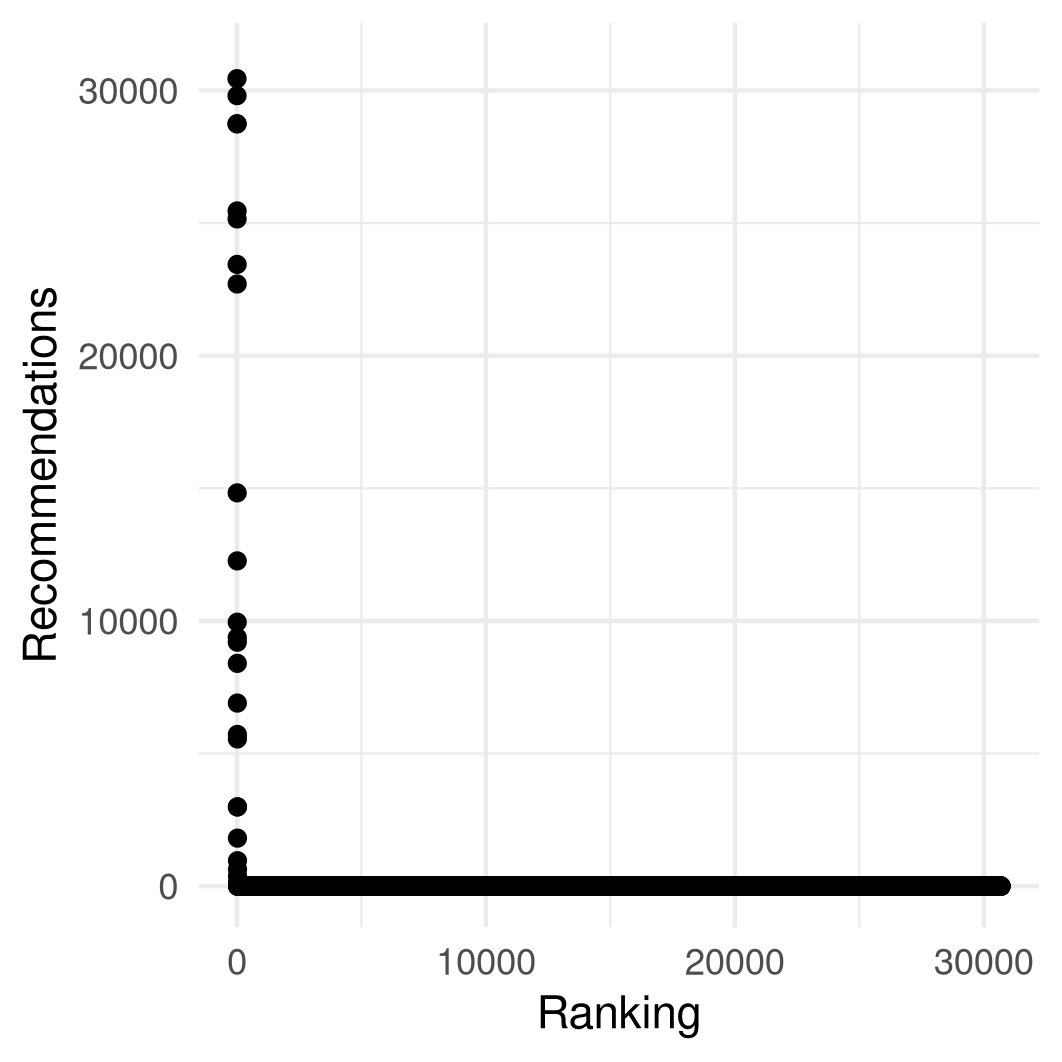
\includegraphics[width=\textwidth]{4b_euclidean}
    \caption{Euclidean distance.\label{fig:fig4b}}
  \end{subfigure}
  \begin{subfigure}{0.3\textwidth}
    \centering
    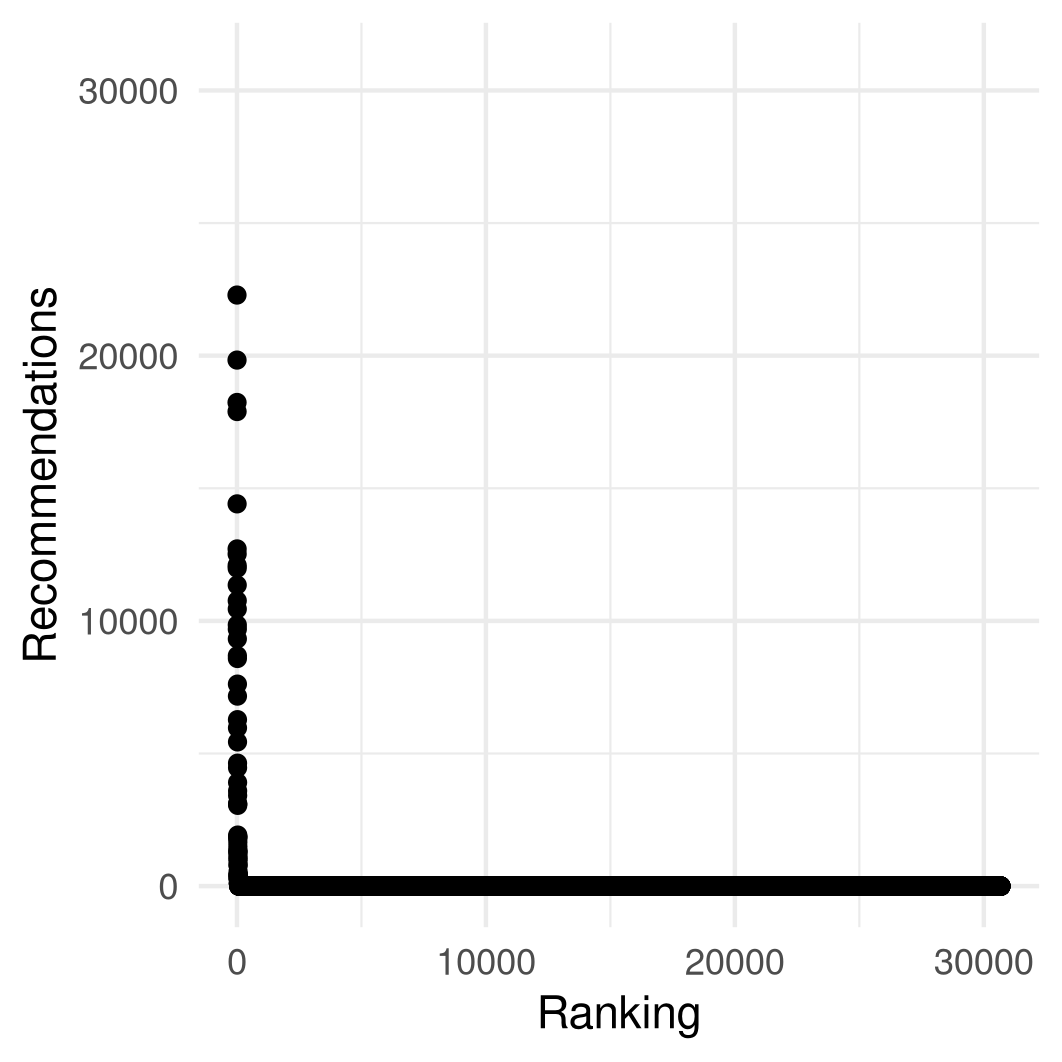
\includegraphics[width=\textwidth]{4c_manhattan}
    \caption{Manhattan distance.\label{fig:fig4c}}
  \end{subfigure}
  \caption{Recommendation profile for cosine (a), euclidean (b), and manhattan
    (c) distances.\label{fig:fig4}}
\end{figure}

At this point it is safe to say that the type of decay seen in recommendation
frequencies up until now is not spurious and must have a clear cause. To better
investigate whether word frequency had an impact on the recommendation profiles
another hypothesis was taken into consideration: do sparser metadata cause the
recommendation curves to display a steep left-hand side?

For the next experiment, each movie was assigned randomly generated metadata,
i.e., each text was comprised of random words sampled uniformly from the full
metadata corpus. The baseline probability of any given word $w_i$ being added to
the metadata of a movie was equal to $\overline{P(w)}$, the average probability
over every word in the original corpus.

In addition to this baseline probability, two extra sets of metadata were
constructed: one where each word was 10 times more likely to be selected than
$\overline{P(w)}$, and another where each word was 100 times more likely. All
three constructed datasets can be concisely described through the expression
$P(w_i) = C \times \overline{P(w)}, C = \{1, 10, 100\}$.

Figure~\ref{fig:fig5} displays the recommendation profiles for each different
$C$. Concretely, the figures are equivalent to creating random metadata for the
movies where the probability of any single word being selected was approximately
$1.54 \times 10^{-4}$, $1.54 \times 10^{-3}$, and $1.54 \times 10^{-2}$
respectively. The results do support the aforementioned hypothesis since less
sparse vectors indeed generated less exponential decays.

\begin{figure}
  \centering
  \begin{subfigure}{0.3\textwidth}
    \centering
    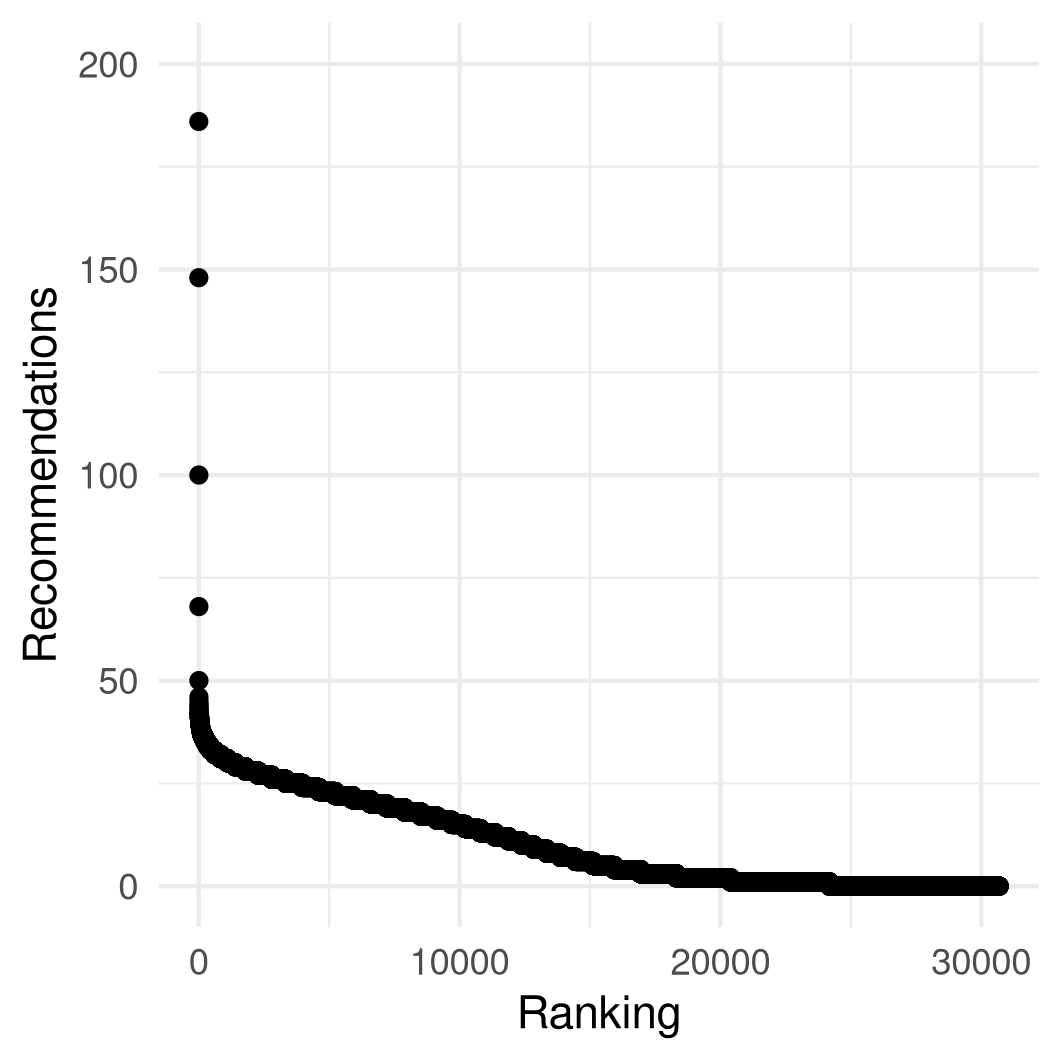
\includegraphics[width=\textwidth]{5a_p}
    \caption{$P(w_{i}) = 1 \times \overline{P(w)}$.\label{fig:fig5a}}
  \end{subfigure}
  \begin{subfigure}{0.3\textwidth}
    \centering
    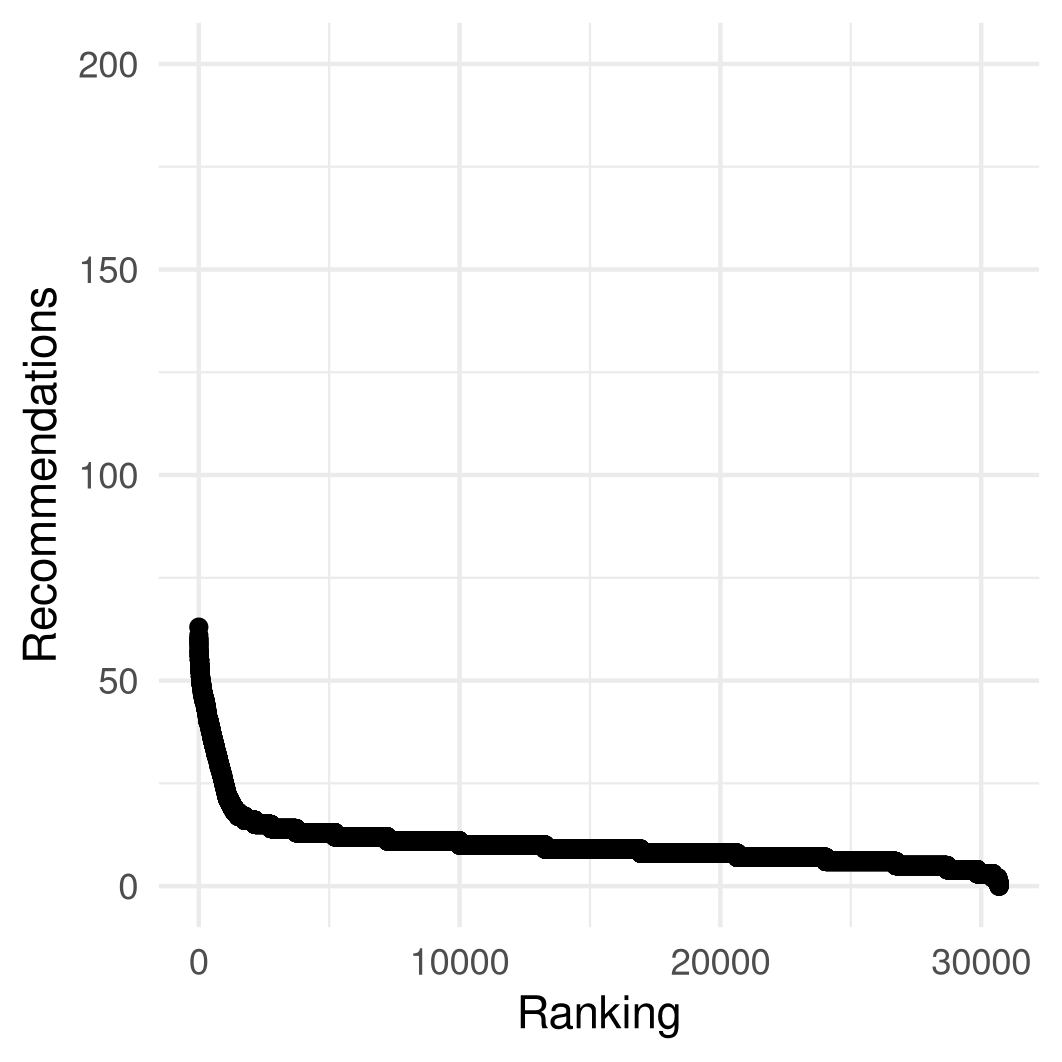
\includegraphics[width=\textwidth]{5b_p10}
    \caption{$P(w_{i}) = 10 \times \overline{P(w)}$.\label{fig:fig5b}}
  \end{subfigure}
  \begin{subfigure}{0.3\textwidth}
    \centering
    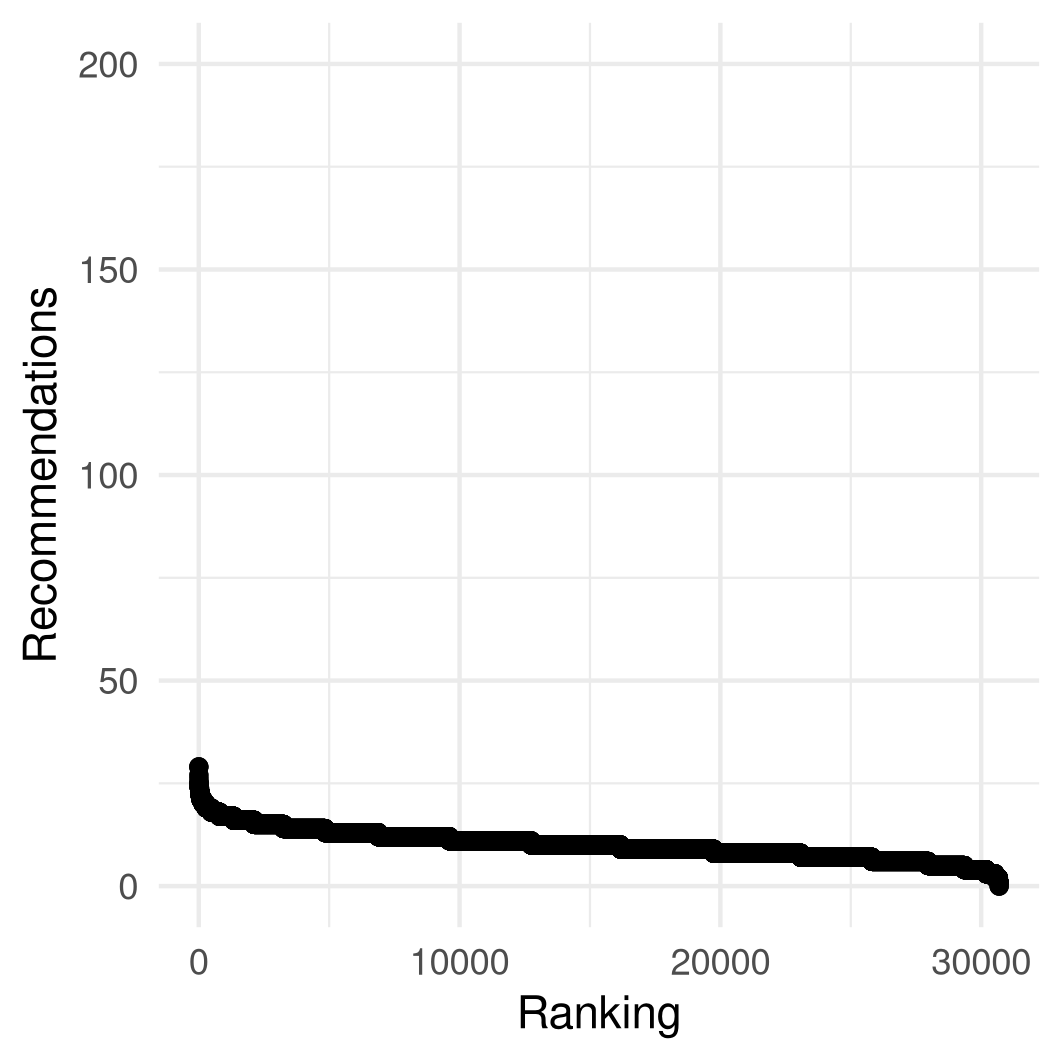
\includegraphics[width=\textwidth]{5c_p100}
    \caption{$P(w_{i}) = 100 \times \overline{P(w)}$.\label{fig:fig5c}}
  \end{subfigure}
  \caption{Recommendation profile of samples with
    $P(w_{i}) = C \times \overline{P(w)}$, $C = 1$ (a), $10$ (b), and $100$
    (c).\label{fig:fig5}}
\end{figure}

\subsection{Sanity Checks}
\label{subsec:sanity03}

After the previous experiments, sanity checks were needed in order to guarantee
that the previous hypothesis was generalizable. The first check should verify
whether an artificial movie created as a combination of the metadata from other
movies favored by the recommendation algorithm would also be favored, while the
second should check whether shorter vectors would change the decay already
observed despite being as sparse as their longer counterparts.

Figure~\ref{fig:fig6} showcases the two sanity checks. Figure~\ref{fig:fig6a}
was a model applied to the vanilla dataset with the addition of the movie
highlighted in red. As expected, this movie also showed up in the
top-recommended subset. Figure~\ref{fig:fig6b} comes from a model applied to
randomly generated vector representations in a similar fashion to the ones in
Figure~\ref{fig:fig5}, except each vector could only have 15,000 elements
instead of 55,681 (as with the vanilla model). The pattern observed before
persisted, meaning that the hypothesis still stood.

\begin{figure}
  \centering
  \begin{subfigure}{0.45\textwidth}
    \centering
    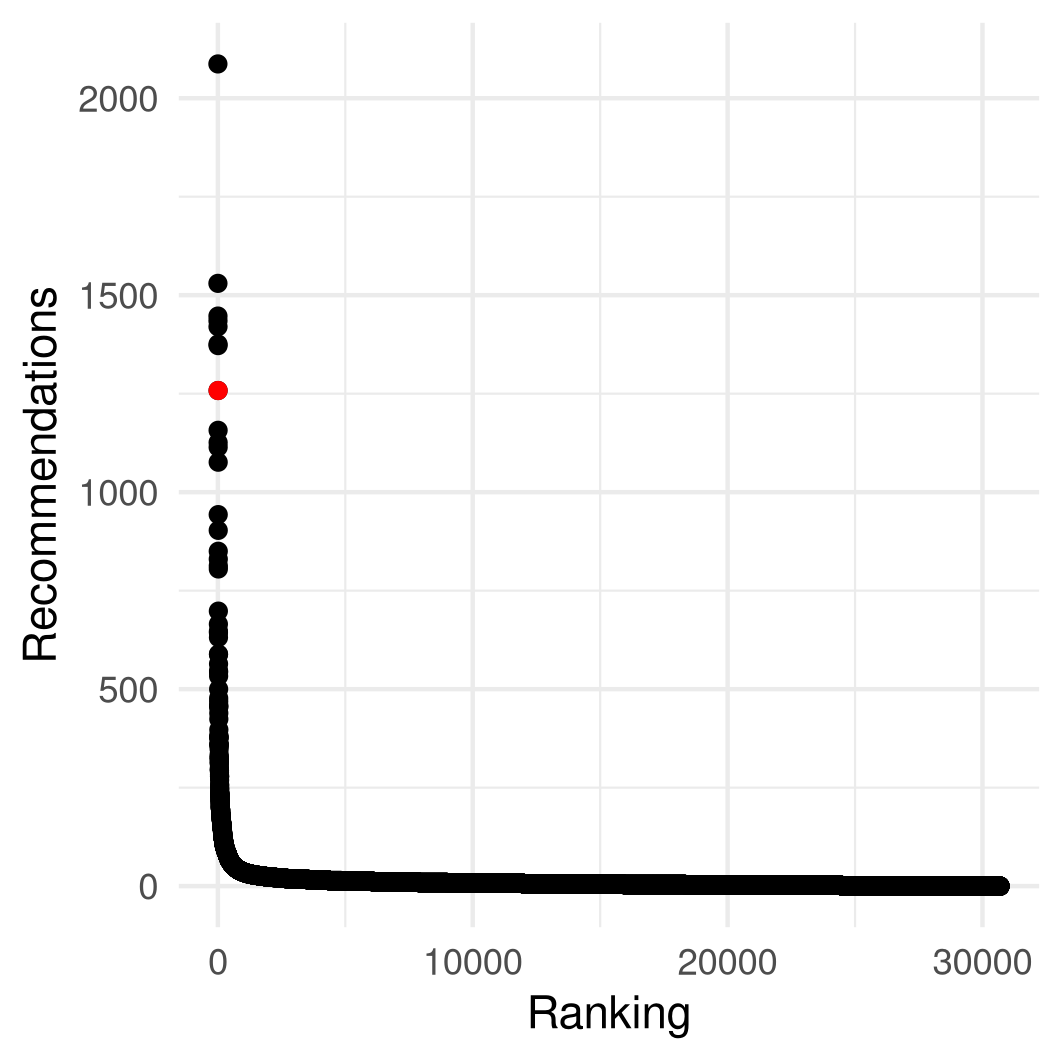
\includegraphics[width=\textwidth]{6a_artificial_movie}
    \caption{Vanilla model with artificial movie in red.\label{fig:fig6a}}
  \end{subfigure}
  \begin{subfigure}{0.45\textwidth}
    \centering
    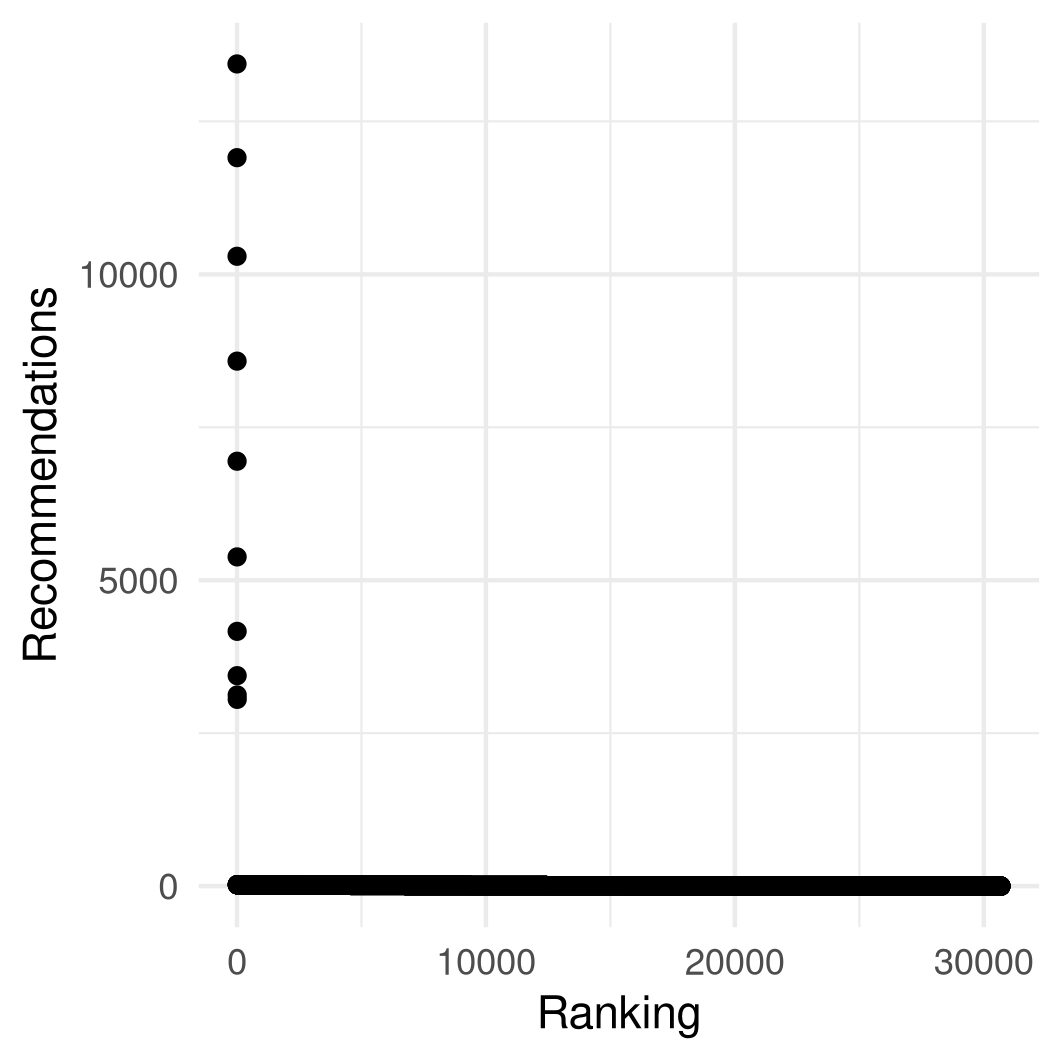
\includegraphics[width=\textwidth]{6b_long}
    \caption{Model with short vector representations.\label{fig:fig6b}}
  \end{subfigure}
  \caption{Recommendation profile for artificial movie (a) and short vector
    representations (b).\label{fig:fig6}}
\end{figure}

The last two models were considered the confirmations of the hypothesis that (at
least for this kind of recommendation systems) a subset of items was always much
more recommended than the rest as long as the data was sparse.
Figure~\ref{fig:fig7a} represents the same recommendation algorithm applied to
another dataset, the Book-Crossing dataset. Figure~\ref{fig:fig7b} contains the
results of the model applied to another set of random vector representations,
this time with the probability of each element being non-zero respecting the
marginal distributions of the vanilla dataset. Again, the exponential decay
pattern persisted, only slightly less pronounced in the Book-Crossing case.

\begin{figure}
  \centering
  \begin{subfigure}{0.45\textwidth}
    \centering
    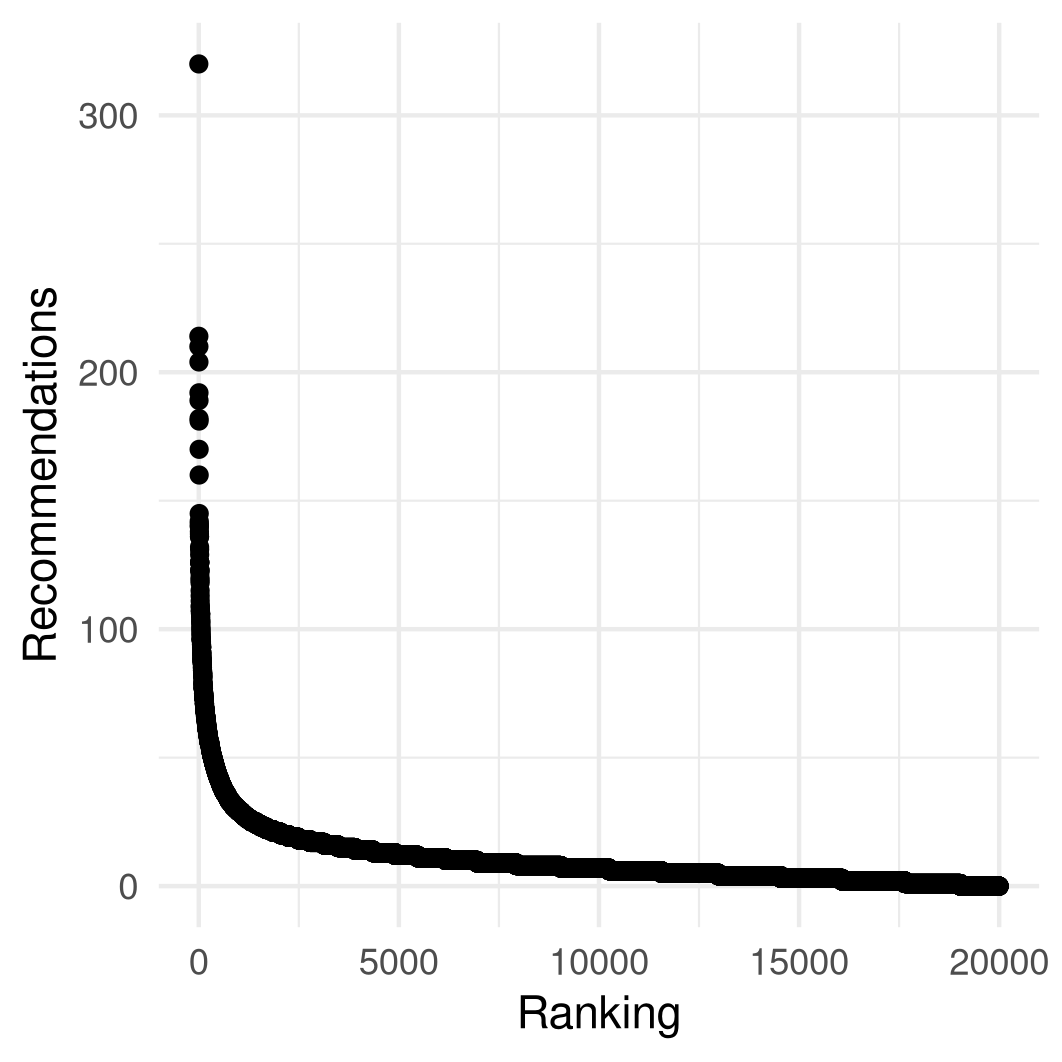
\includegraphics[width=\textwidth]{7a_books}
    \caption{Recommendation profile for book dataset.\label{fig:fig7a}}
  \end{subfigure}
  \begin{subfigure}{0.45\textwidth}
    \centering
    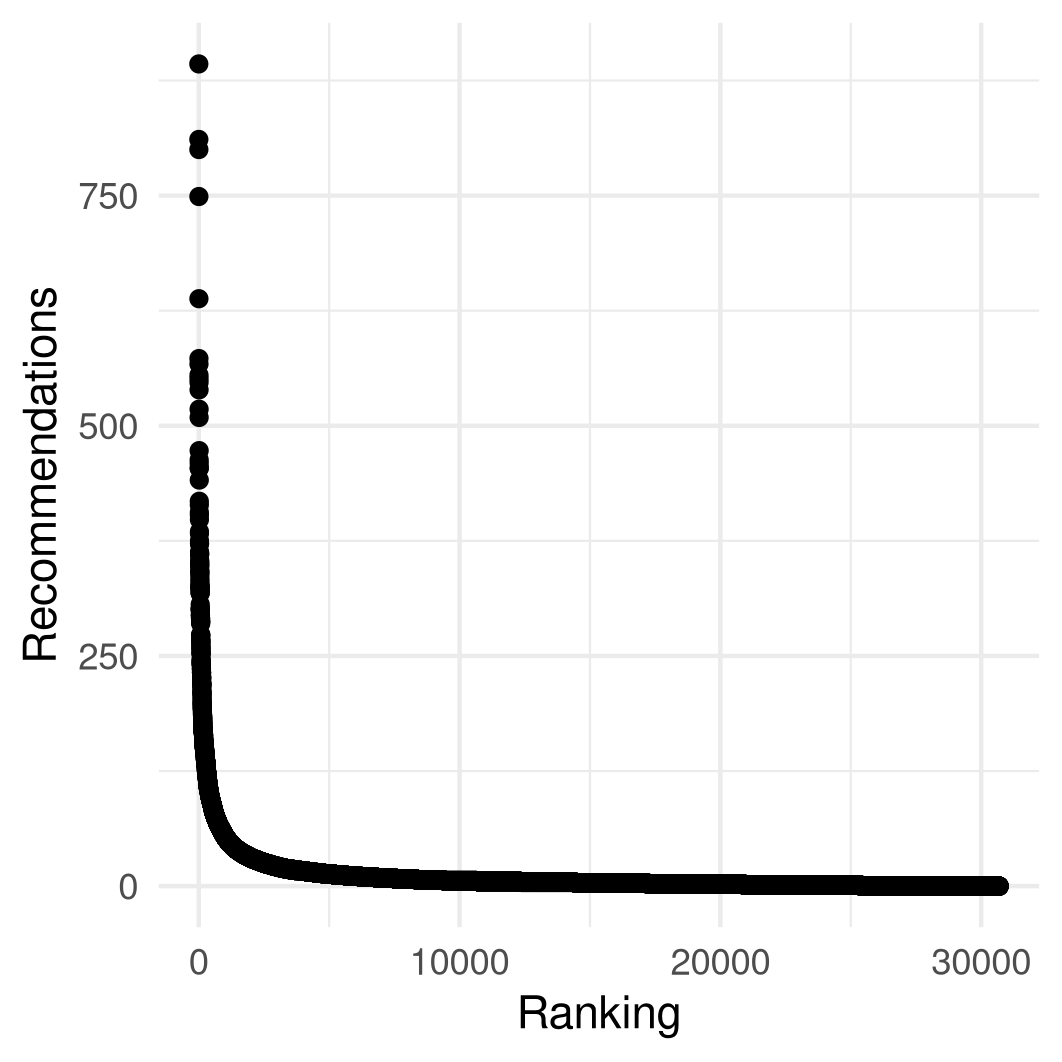
\includegraphics[width=\textwidth]{7b_mimic}
    \caption{Random simularion of vanilla.\label{fig:fig7b}}
  \end{subfigure}
  \caption{Recommendation profile for book dataset (a) and random simulation of
    vanilla (b).\label{fig:fig7}}
\end{figure}

The analysis up until now has been static, that is, the recommendation model
does not learn from the users' responses to its suggestions. There is no
interaction with users and no opportunity to evolve over time. The next chapter
addresses this point by using Google's newly released TensorFlow Recommenders
library \citep{noauthor_tensorflow_nodate} to gather data about what happens to
a system's recommendations as users follow its suggestions. Employing a deep
learning model that is able to improve over time is a significant departure from
the content-based models presented here and, if a similar recommendation profile
can also be detected for multi-criteria recommender systems on dynamic
scenarios, then the hypothesis ventilated in the section above would become even
more plausible.
